\documentclass{jsarticle}
\usepackage[dvipdfmx]{graphicx}
\usepackage{float}
\usepackage{amsmath}
\usepackage[dvipdfmx]{color}
\usepackage{listings}
\usepackage{subfigure}
\begin{document}
\title{小野寺研インターン}
\author{澤 孝晃}
\maketitle

\section{序論}

トランジスタの微細化によりゲート長が7nmのデバイスが製造可能となっており、μm以下の寸法になってからは電子や分子の量子的な揺らぎが顕著になり、大量のトランジスタからなら集積回路のチップにおいて、同じ寸法のトランジスタ特性間にミスマッチが起きるようになった。ここで、素子同士の特性のミスマッチが回路の性能と信頼性にどう影響を与えるのかが重要である。製造時に発生する特性のミスマッチは静的ばらつきと認識されている一方、動作時にトランジスタの特性が時間によって変動することがありノイズや経年劣化として認識されている。ノイズの主要成分は熱雑音であり白色雑音とも呼ばれる。

主要成分の他に、結晶と結晶の界面に置いて、分子間結合の分子間結合の切断による欠陥が存在する。界面に存在する欠陥に自由キャリアの捕獲と放出が繰り返されると電流の時間変動が発生する。このような変動をフリッカーノイズと呼び、低い周波数領域に置いてパワー密度が大きいことが特徴である。MOSトランジスタの場合、シリコンと酸化膜の間の界面に存在する欠陥が原因となっている。トランジスタの寸法がμm以下になってから、各種欠陥へのキャリアのトラップによる影響が顕著に現れ始めた。その理由として、欠陥1つへのキャリアのトラップの相対的な影響が顕著にあらわれたことと、製造技術の進歩により各種欠陥の数が減少してきており、あるトランジスタに欠陥が存在する確率が減少してきたことがある。従って、1つの欠陥がチャネルに流れる電流にどう影響されるか正確に見積もる手法が求められるようになった。相対的に大きな電流変動は、1つの欠陥への1つの欠陥へのキャリアの捕獲と放出の減少により発生するため離散的な変動として観測される。また、その変動が起きる時間間隔は固定ではなく大きくばらつく。

ランダムテレグラフノイズ(RTN)は界面に存在するトラップにキャリアの捕獲・放出によりデバイスの閾値電圧が変動する現象である。閾値電圧だけでなく移動度が変化する説もある。RTNを特徴付けるパラメータは、トラップあたりのオン電流の変化量、トラップあたりの時定数、トラップの数の3種類がある。トラップあたりのRTNパラメータを評価するのではなく、RTNによる合計量の変動を評価し、その変動量の分布をモデル化することにより回路設計に活かすことを目標にする。

今回のインターンでは、微細デバイスに発生するRTNをリング発振回路を用いて測定し、RTNが回路性能の最悪分布に与える影響を評価する。測定対象であるRTNは統計的な性質を持っており、各種統計的な性質をモデル化することが目的である。統計的な評価を行うために、同じ寸法の大量のデバイスの電流特性の時間変化を測定し、デバイス毎に観測される電流値変動の振幅および捕獲・放出するまでの平均時間などを評価する。

\section{方法}

今回の測定環境では、FPGAボードとPCを使って、スロット0からスロット71のリングオシレータ(RO)を、セクション0からセクション383まで384個のセクションの発信周波数を測定する。各セクション10秒ずつ測定するので、合計1時間程度かかる。また、ROの電源は0.5Vに設定する。

\section{結果}



\section{N skewedの結果}

分周した発振周波数のqqplotを描く。qqpoltとは得られたデータと理論分布を比較し、その類似度を調べるためのグラフである。横軸は各分周器にかけられた発振周波数の各セクションでの最大値と最小値の差を最大値で割った値である。縦軸は理論分位数となっている。

\begin{figure}[H]
	\centering
	\subfigure[p=655の時のqqplot]{
		\includegraphics[width=10cm]{../../images/anotation/p655.pdf}
		\label{fig:p655_qqplot}
	}
	\subfigure[p=655の時の傾きと切片]{
		\includegraphics[width=4cm]{../../least_squares/p655.png}
		\label{fig:p665_slope_intercept}
	}
	\subfigure[p=655, n=2240の時の波形]{
		\includegraphics[width=14cm]{../../images/waveform/p655.pdf}
		\label{fig:p665_waveform}
	}
	\caption{the effect of the edge length of FET in p = 655}
	\label{fig:the_effect_of_the_edge_length_of_fet_in_p_655}
\end{figure}


\section{P skewedの結果}

\begin{figure}[H]
	\centering
	\subfigure[n=420の時のqqplot]{
		\includegraphics[width=10cm]{../../images/anotation/n420.pdf}
		\label{fig:n420_qqplot}
	}
	\subfigure[n=420の時の傾きと切片]{
		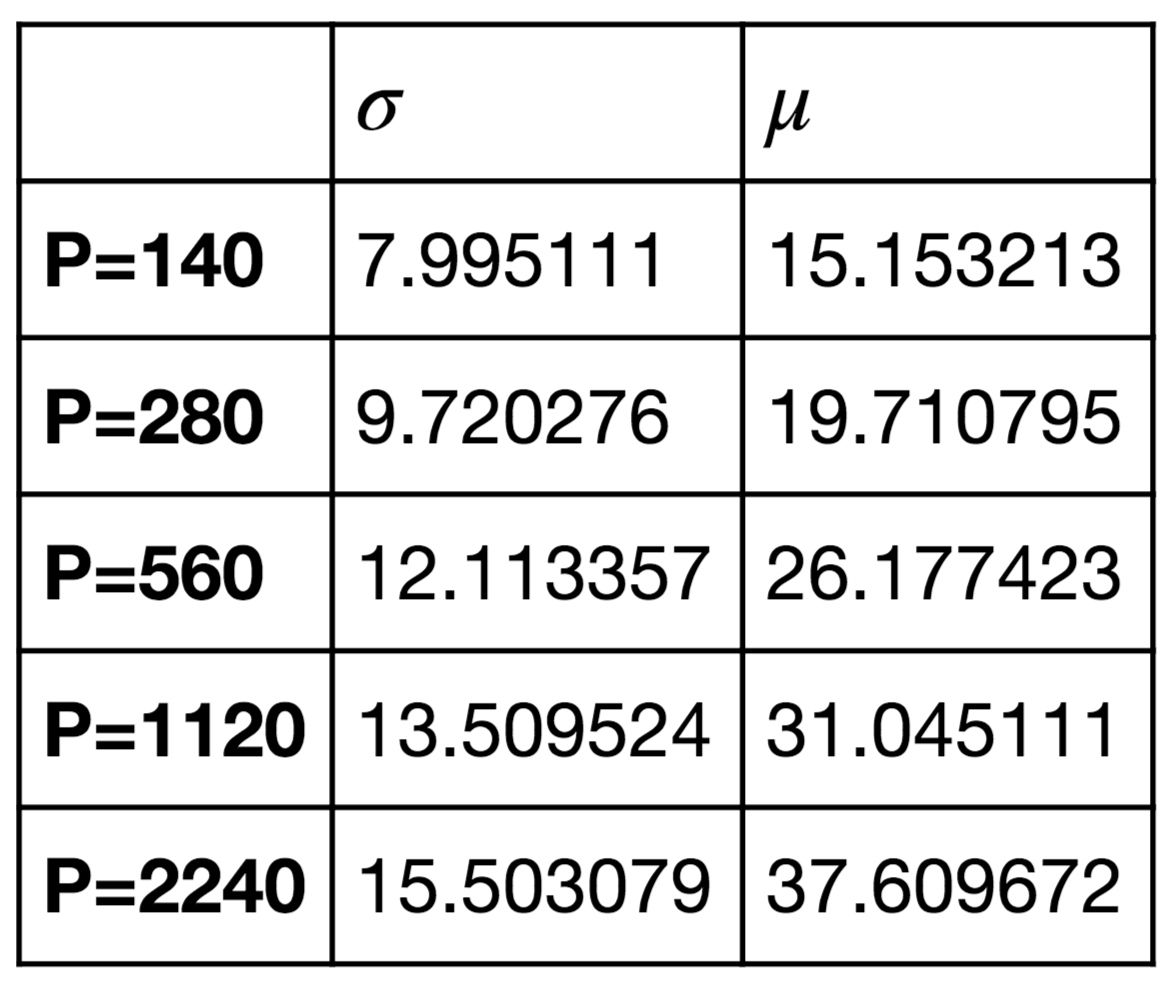
\includegraphics[width=4cm]{../../least_squares/n420.png}
		\label{fig:n420_slope_intercept}
	}
	\subfigure[n=420, p=2240の時の波形]{
		\includegraphics[width=14cm]{../../images/waveform/n420.pdf}
		\label{fig:n420_waveform}
	}
	\caption{the effect of the edge length of FET in n = 420}
	\label{fig:the_effect_of_the_edge_length_of_fet_in_n_420}
\end{figure}


\section{Balancedの結果}

\begin{figure}[H]
	\centering
	\subfigure[Balancedの時のqqplot]{
		\includegraphics[width=10cm]{../../images/anotation/square.pdf}
		\label{fig:balanced_qqplot}
	}
	\subfigure[Balancedの時の傾きと切片]{
		\includegraphics[width=4cm]{../../least_squares/square.png}
		\label{fig:balanced_slope_intercept}
	}
	\subfigure[n,p=2240の時の波形]{
		\includegraphics[width=14cm]{../../images/waveform/square.pdf}
		\label{fig:balanced_waveform}
	}
	\caption{the effect of the size of FET}
	\label{fig:the_effect_of_the_size_of_fet}
\end{figure}


\section{stageの結果}

\begin{figure}[H]
	\centering
	\subfigure[stageの時のqqplot]{
		\includegraphics[width=10cm]{../../images/anotation/stage.pdf}
		\label{fig:stage_qqplot}
	}
	\subfigure[stageの時の傾きと切片]{
		\includegraphics[width=4cm]{../../least_squares/stage.png}
		\label{fig:stage_slope_intercept}
	}
	\subfigure[stage=59の時の波形]{
		\includegraphics[width=14cm]{../../images/waveform/stage.pdf}
		\label{fig:stage_waveform}
	}
	\caption{the effect of the stage of FET}
	\label{fig:the_effect_of_the_stage_of_fet}
\end{figure}


\section{extra loadの結果}

\begin{figure}[H]
	\centering
	\subfigure[extra loadの時のqqplot]{
		\includegraphics[width=10cm]{../../images/anotation/load.pdf}
		\label{fig:load_qqplot}
	}
	\subfigure[extra loadの時の傾きと切片]{
		\includegraphics[width=4cm]{../../least_squares/load.png}
		\label{fig:load_slope_intercept}
	}
	\subfigure[load=largeの時の波形]{
		\includegraphics[width=14cm]{../../images/waveform/load.pdf}
		\label{fig:load_waveform}
	}
	\caption{the effect of the extra load of FET}
	\label{fig:the_effect_of_the_extra_load_of_fet}
\end{figure}




% \section{正規化前の結果}
% \subsection{ヒストグラム}
% まず、発振周波数のヒストグラムを描く。横軸は分周器にかけられた発振周波数で縦軸はその周波数を示した回数である。図\ref{fig:fig_max_hist/180518_ch02v050r0d3_int252_time10000_fig_max_hist.pdf}は$p=655, n=140$の時のヒストグラムであり、正規分布に従っていることが予想できる。

% \begin{figure}[H]
% 	\centering
% 	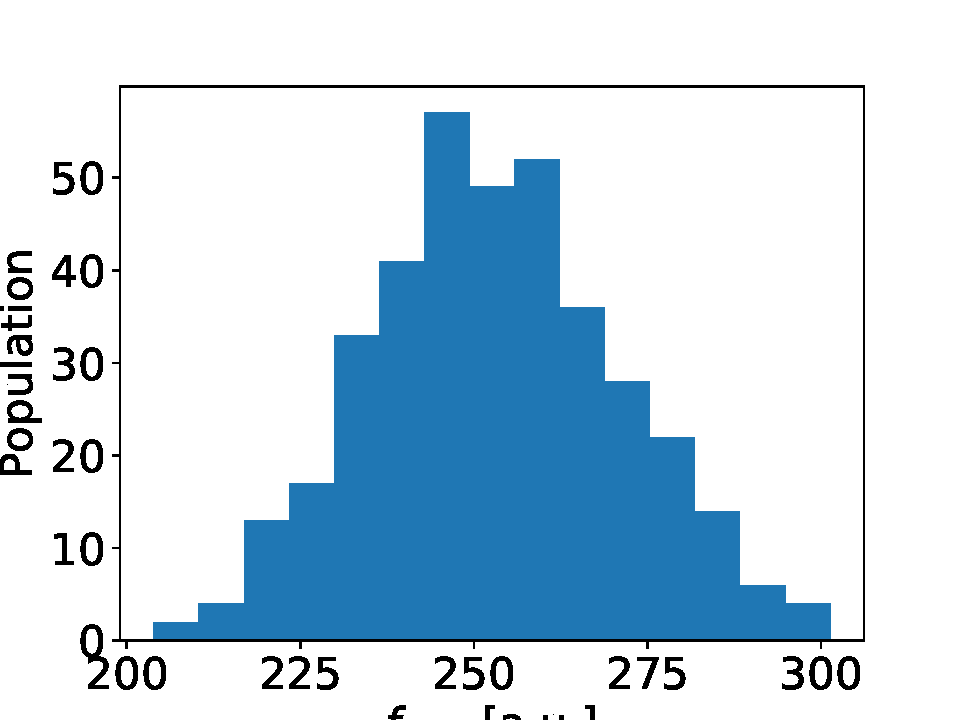
\includegraphics[width=8cm]{../../images/fig_max_hist/180518_ch02v050r0d3_int252_time10000_fig_max_hist.pdf}
% 	\label{fig:fig_max_hist/180518_ch02v050r0d3_int252_time10000_fig_max_hist.pdf}
% 	\caption{Histogram before normalization}
% \end{figure}

% \subsection{qq-plot}
% 次に、発振周波数のqqplotを描く。qqpoltとは得られたデータと理論分布を比較し、その類似度を調べるためのグラフである。横軸は分周期にかけられた

% \begin{figure}[H]
% 	\centering
% 	\includegraphics[width=8cm]{../../images/fig_max_qqplot/180518_ch02v050r0d3_int252_time10000_fig_max_qqplot.pdf}
% 	\label{fig:fig_max_qqplot/180518_ch02v050r0d3_int252_time10000_fig_max_qqplot.pdf}
% \end{figure}

% \section{正規化後の結果}
% \subsection{ヒストグラム}
% まず、発振周波数のヒストグラムを描く。横軸は各分周器にかけられた発振周波数の各セクションでの最大値と最小値の差を最大値で割った値である。縦軸はその周波数を示した回数である。図\ref{fig:fig_delta_hist/180518_ch02v050r0d3_int252_time10000_fig_delta_hist.pdf}は$p=655, n=140$の時のヒストグラムである。

% \begin{figure}[H]
% 	\centering
% 	\includegraphics[width=10cm]{../../images/fig_delta_hist/180518_ch02v050r0d3_int252_time10000_fig_delta_hist.pdf}
% 	\label{fig:fig_delta_hist/180518_ch02v050r0d3_int252_time10000_fig_delta_hist.pdf}
% 	\caption{Histogram of frequency after normalized}
% \end{figure}

% \begin{figure}[H]
% 	\centering
% 	\subfigure[7段]{
% 		\includegraphics[width=5cm]{../../images/fig_delta_hist/180522_ch02v050r36d3_int247_time10000_fig_delta_hist.pdf}
% 		\label{fig:fig_delta_qqplot/180522_ch02v050r36d3_int247_time10000_fig_delta_qqplot.pdf}
% 	}
% 	\subfigure[13段]{
% 		\includegraphics[width=5cm]{../../images/fig_delta_hist/180522_ch02v050r41d3_int163_time10000_fig_delta_hist.pdf}
% 		\label{fig:fig_delta_qqplot/180522_ch02v050r41d3_int163_time10000_fig_delta_qqplot.pdf}
% 	}
% 	\subfigure[19段]{
% 		\includegraphics[width=5cm]{../../images/fig_delta_hist/180522_ch02v050r42d3_int114_time10000_fig_delta_hist.pdf}
% 		\label{fig:fig_delta_qqplot/180522_ch02v050r42d3_int114_time10000_fig_delta_qqplot.pdf}
% 	}
% 	\subfigure[29段]{
% 		\includegraphics[width=5cm]{../../images/fig_delta_hist/180522_ch02v050r43d3_int75_time10000_fig_delta_hist.pdf}
% 		\label{fig:fig_delta_qqplot/180522_ch02v050r43d3_int75_time10000_fig_delta_qqplot.pdf}
% 	}
% 	\subfigure[59段]{
% 		\includegraphics[width=5cm]{../../images/fig_delta_hist/180522_ch02v050r44d3_int41_time10000_fig_delta_hist.pdf}
% 		\label{fig:number_of_network_operations_comparison_5}
% 	}
% 	\caption{Number of network operations comparison}
% 	\label{fig:number_of_network_operations_comparison}
% \end{figure}

% \subsection{qq-plot}
% 次に、発振周波数のqqplotを描く。qqpoltとは得られたデータと理論分布を比較し、その類似度を調べるためのグラフである。横軸は各分周器にかけられた発振周波数の各セクションでの最大値と最小値の差を最大値で割った値である。縦軸は理論分位数となっている。

% \begin{figure}[H]
% 	\centering
% 	\subfigure[p=655]{
% 		\includegraphics[width=10cm]{../../images/none_anotation/p655.pdf}
% 		\label{fig:p655}
% 	}
% 	\subfigure[n=420]{
% 		\includegraphics[width=10cm]{../../images/none_anotation/n420.pdf}
% 		\label{fig:n420}
% 	}
% 	\caption{the effect of the edge length of FET}
% 	\label{fig:the_effect_of_the_size_of_fet}
% \end{figure}

% 図\ref{fig:the_effect_of_the_size_of_fet}はFETの1辺の長さを変化させた時の結果である。どのスロットの値も正規分布に従っていて、FETの面積が大きくなればなるほど$\Delta F / F_max$の値は小さくなることがわかる。

% \begin{figure}[H]
% 	\centering
% 	\includegraphics[width=10cm]{../../images/square.pdf}
% 	\label{fig:square}
% 	\caption{the effect of the area of FET}
% \end{figure}

% 図\ref{fig:square}はFETの両辺の長さを変化させた時の結果である。1辺を変化させた時の結果と似ているが、FETの面積が小さい時に理論分布との類似度が下がっていると考察する。

% \begin{figure}[H]
% 	\centering
% 	\includegraphics[width=10cm]{../../images/stage.pdf}
% 	\label{fig:stage}
% 	\caption{the effect of the number of stages}
% \end{figure}

% 図\ref{fig:stage}はリングオシレーターの段数を変化させた時の結果である。段数が大きくなればなるほど$\Delta F / F_max$の値は小さくなることがわかる。また、それぞれのセクションにて$\Delta F / F_max$が大きいところで理論分布との類似度が下がっていると考察する。



\end{document}
